\documentclass{beamer}
\usetheme{default}
\useoutertheme{miniframes}
\useinnertheme{circles}
\usepackage{listings}
\usepackage{xcolor}
\usepackage{bookmark}
\usepackage{url}

% Reusable Navy theme
% =============================================
% NAVY THEME FOR BEAMER
% Reusable theme: \input this file after \documentclass{beamer} and base theme.
% =============================================

% COLOR SCHEME: Professional Navy
\definecolor{NavyDark}{RGB}{20, 40, 80}        % Deep navy
\definecolor{NavyMid}{RGB}{40, 65, 115}        % Medium navy
\definecolor{NavyLight}{RGB}{70, 100, 150}     % Lighter navy accent

% Main structure color
\setbeamercolor{structure}{fg=NavyDark}

% Header (top navigation bar)
\setbeamercolor{section in head/foot}{fg=white, bg=NavyDark}
\setbeamercolor{subsection in head/foot}{fg=white, bg=NavyMid}

% Footer colors (subtle gradient)
\setbeamercolor{author in head/foot}{fg=white, bg=NavyLight}
\setbeamercolor{title in head/foot}{fg=white, bg=NavyMid}
\setbeamercolor{date in head/foot}{fg=white, bg=NavyDark}

% Title page
\setbeamercolor{title}{fg=NavyDark}
\setbeamercolor{subtitle}{fg=NavyMid}
\setbeamercolor{author}{fg=NavyDark!80}
\setbeamercolor{date}{fg=NavyDark!60}

% Frame titles
\setbeamercolor{frametitle}{fg=white, bg=NavyDark}
\setbeamercolor{framesubtitle}{fg=NavyMid}

% Itemize/enumerate
\setbeamercolor{item}{fg=NavyDark}
\setbeamercolor{subitem}{fg=NavyMid}

% Navigation dots
\setbeamercolor{mini frame}{fg=white, bg=white!30}
\setbeamercolor{mini frame inactive}{fg=white!50}

% Custom footline: Author | Short Title | Date + Frame Number
\setbeamertemplate{footline}{
  \leavevmode%
  \hbox{%
  \begin{beamercolorbox}[wd=.20\paperwidth,ht=2.5ex,dp=1ex,left,leftskip=1em]{author in head/foot}%
    \usebeamerfont{author in head/foot}\insertshortauthor
  \end{beamercolorbox}%
  \begin{beamercolorbox}[wd=.55\paperwidth,ht=2.5ex,dp=1ex,center]{title in head/foot}%
    \usebeamerfont{title in head/foot}\insertshorttitle
  \end{beamercolorbox}%
  \begin{beamercolorbox}[wd=.25\paperwidth,ht=2.5ex,dp=1ex,right,rightskip=1em]{date in head/foot}%
    \usebeamerfont{date in head/foot}\insertshortdate{}\hspace*{2em}
    \insertframenumber{} / \inserttotalframenumber
  \end{beamercolorbox}}%
  \vskip0pt%
}

% Code listing style (optional; requires \usepackage{listings} in main doc)
\lstset{
    basicstyle=\ttfamily\footnotesize,
    breaklines=true,
    frame=single,
    backgroundcolor=\color{gray!10},
}


% ============================================
% TITLE BLOCK
% ============================================
\title[Using AI as a \textit{Junior} Dev]{Using AI to Build as a \textit{Junior} Developer}
\subtitle{and the many existential questions that come with it}
\author[Sneha S]{Sneha S}
\date{March 7, 2026}

\begin{document}

\maketitle

% ============================================
% SECTION 1: CONTEXT & APPROACH (3-4 mins)
% ============================================
\section{Context}

\begin{frame}{What I'm gonna talk about}
    \begin{itemize}
        \item Context: A little about me
        \item 2 cases: A weekend project \& an actual feature
        \item What's worked for me and what hasn't
        \item What now? And what are the implications for non-developers, and how does that change the way we build?
    \end{itemize}

    \pause
    \vspace{1em}
    \footnotesize
    This talk, as much as it's about how I'm ``using AI'', is also about the many feelings and questions that it has brought out in me and my peers. Hopefully we'll get to talk about those things as well.

    \vspace{2em}
    \scriptsize
    I've done my best to write this presentation by myself. All em-dashes are mine. I took help with the theme though. Available at: \url{saisneha.com/links/ttt-2026-03}


\end{frame}


\begin{frame}{About Me}

    \begin{itemize}[<+->]
    \item I'm actually a biologist by training. I graduated from my masters only in 2022.
    \item I've been pivoting slowly into development over the last 4 years. So this is all actually very new for me.
    \item Not worked in a production software org till recently, a science/data science focused team.
    \end{itemize}

\end{frame}




% ============================================
% SECTION 2: PROJECT 1 - AUTH SOLUTION (5-6 mins)
% ============================================
\section{Weekend Project: Auth}




\begin{frame}{The Auth Problem}
    \begin{itemize}[<+->]
        \item Teammates often want to share a KB, dashboard, or toolkit internally/with collaborators, and they need auth. All users don't have Google accounts.
        \item It's a repeated problem; we reimplement hacky solutions again and again, sometimes insecure ones.
        \item I wanted a simple, replicable system for the org and external collaborators
        \item Every solution felt too daunting or complex to set up (Keycloak comes to mind; ironically, it might not be as complex to set up now)
    \end{itemize}
\end{frame}

\begin{frame}[fragile]{The Initial Prompt}
    \small
    \begin{lstlisting}
Help me build a simple passwordless auth layer for my 
documentation site. It should allow users to login 
using email OTPs or passkeys.

Use Astro for the frontend. Store all user data in a 
SQLite database, but support postgres url as well. Use 
FastAPI for the backend. It should support AWS SES and 
SMTP. Use an env file to keep all secrets separate, 
and put the secrets required in a README.

We'll eventually add Google SSO as well.

    \end{lstlisting}

    \vspace{0.5em}
    \normalsize
    With this, and some additional prompting, I got something working in under 2 hours. Many major aspects, including passkeys and SMTP support - were one-shotted!. 
\end{frame}

\begin{frame}{And then?}
    After the MVP worked, I realized I wanted this auth layer \textbf{shared} across the org and by external collaborators. I didn't want to have to manage multiple auth layers for each app. (This seems so incredibly basic in retrospect, but I did not think of it at all in the first prompt.)

    \pause
    \vspace{1em}
    \textbf{So then, I:}
    \begin{itemize}[<+->]
        \item Had Claude throw together a summary of the repo.
        \item Used the chat interface to discuss the summary and what the point of even building this is, even as a small indie product for mostly myself.
        \item Made a TODO list of what I wanted to build, and then picked up items one by one when I got free time.
    \end{itemize}

\end{frame}

\begin{frame}{"Product" Discussion}

    \vspace{0.5em}
    \textit{Midway, I felt I was getting sucked into a weekend project that would just not be used tomorrow: Should I even continue, or use an existing service, based on my requirements?}

    \vspace{1em}
    \small
    Maybe it was the model's sycophancy but after a bit of back and forth - it said that it does make sense to build this. (I think it only works \textbf{because} I wasn't writing it by hand.)

    \textit{Total time spent: \textasciitilde44 hours (5.5 working days)}

    \vspace{1em}
    GitHub Repo: \url{saisneha.com/links/gatekeeper}

\end{frame}

\begin{frame}{Login Screen}
    \centering
    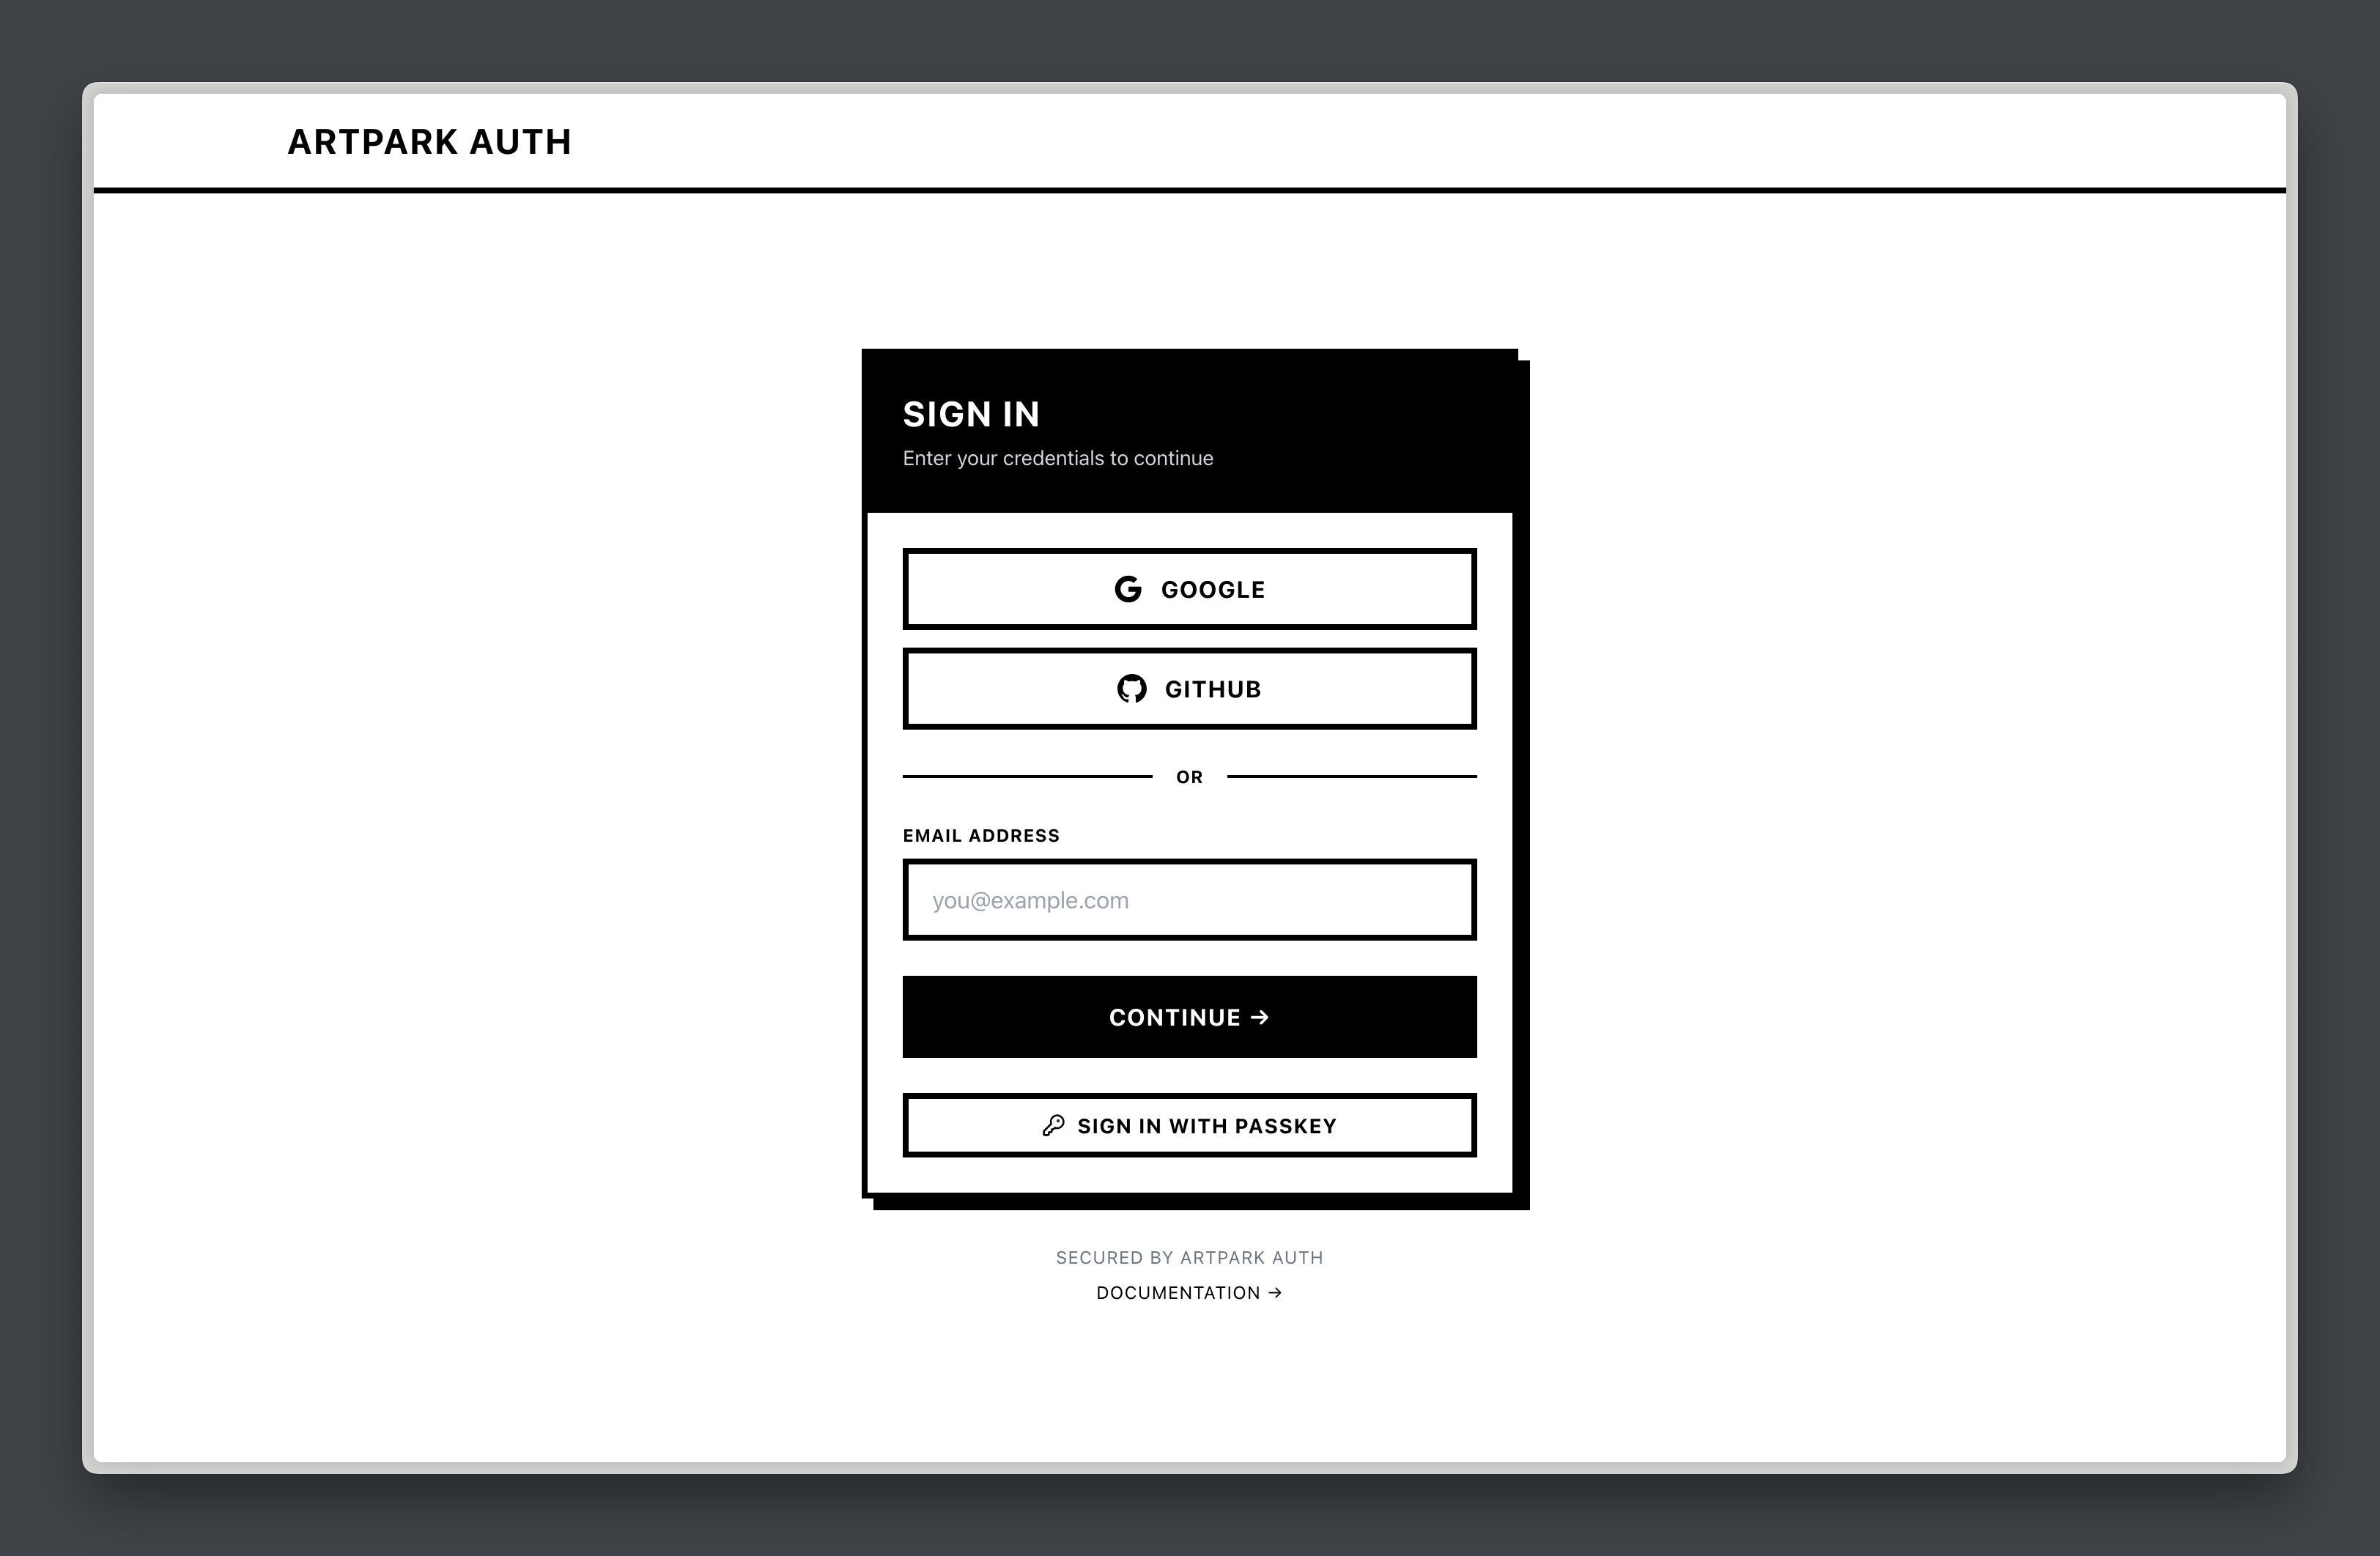
\includegraphics[height=0.85\textheight]{images/login screen.png}
\end{frame}

\begin{frame}{Security Settings}
    \centering
    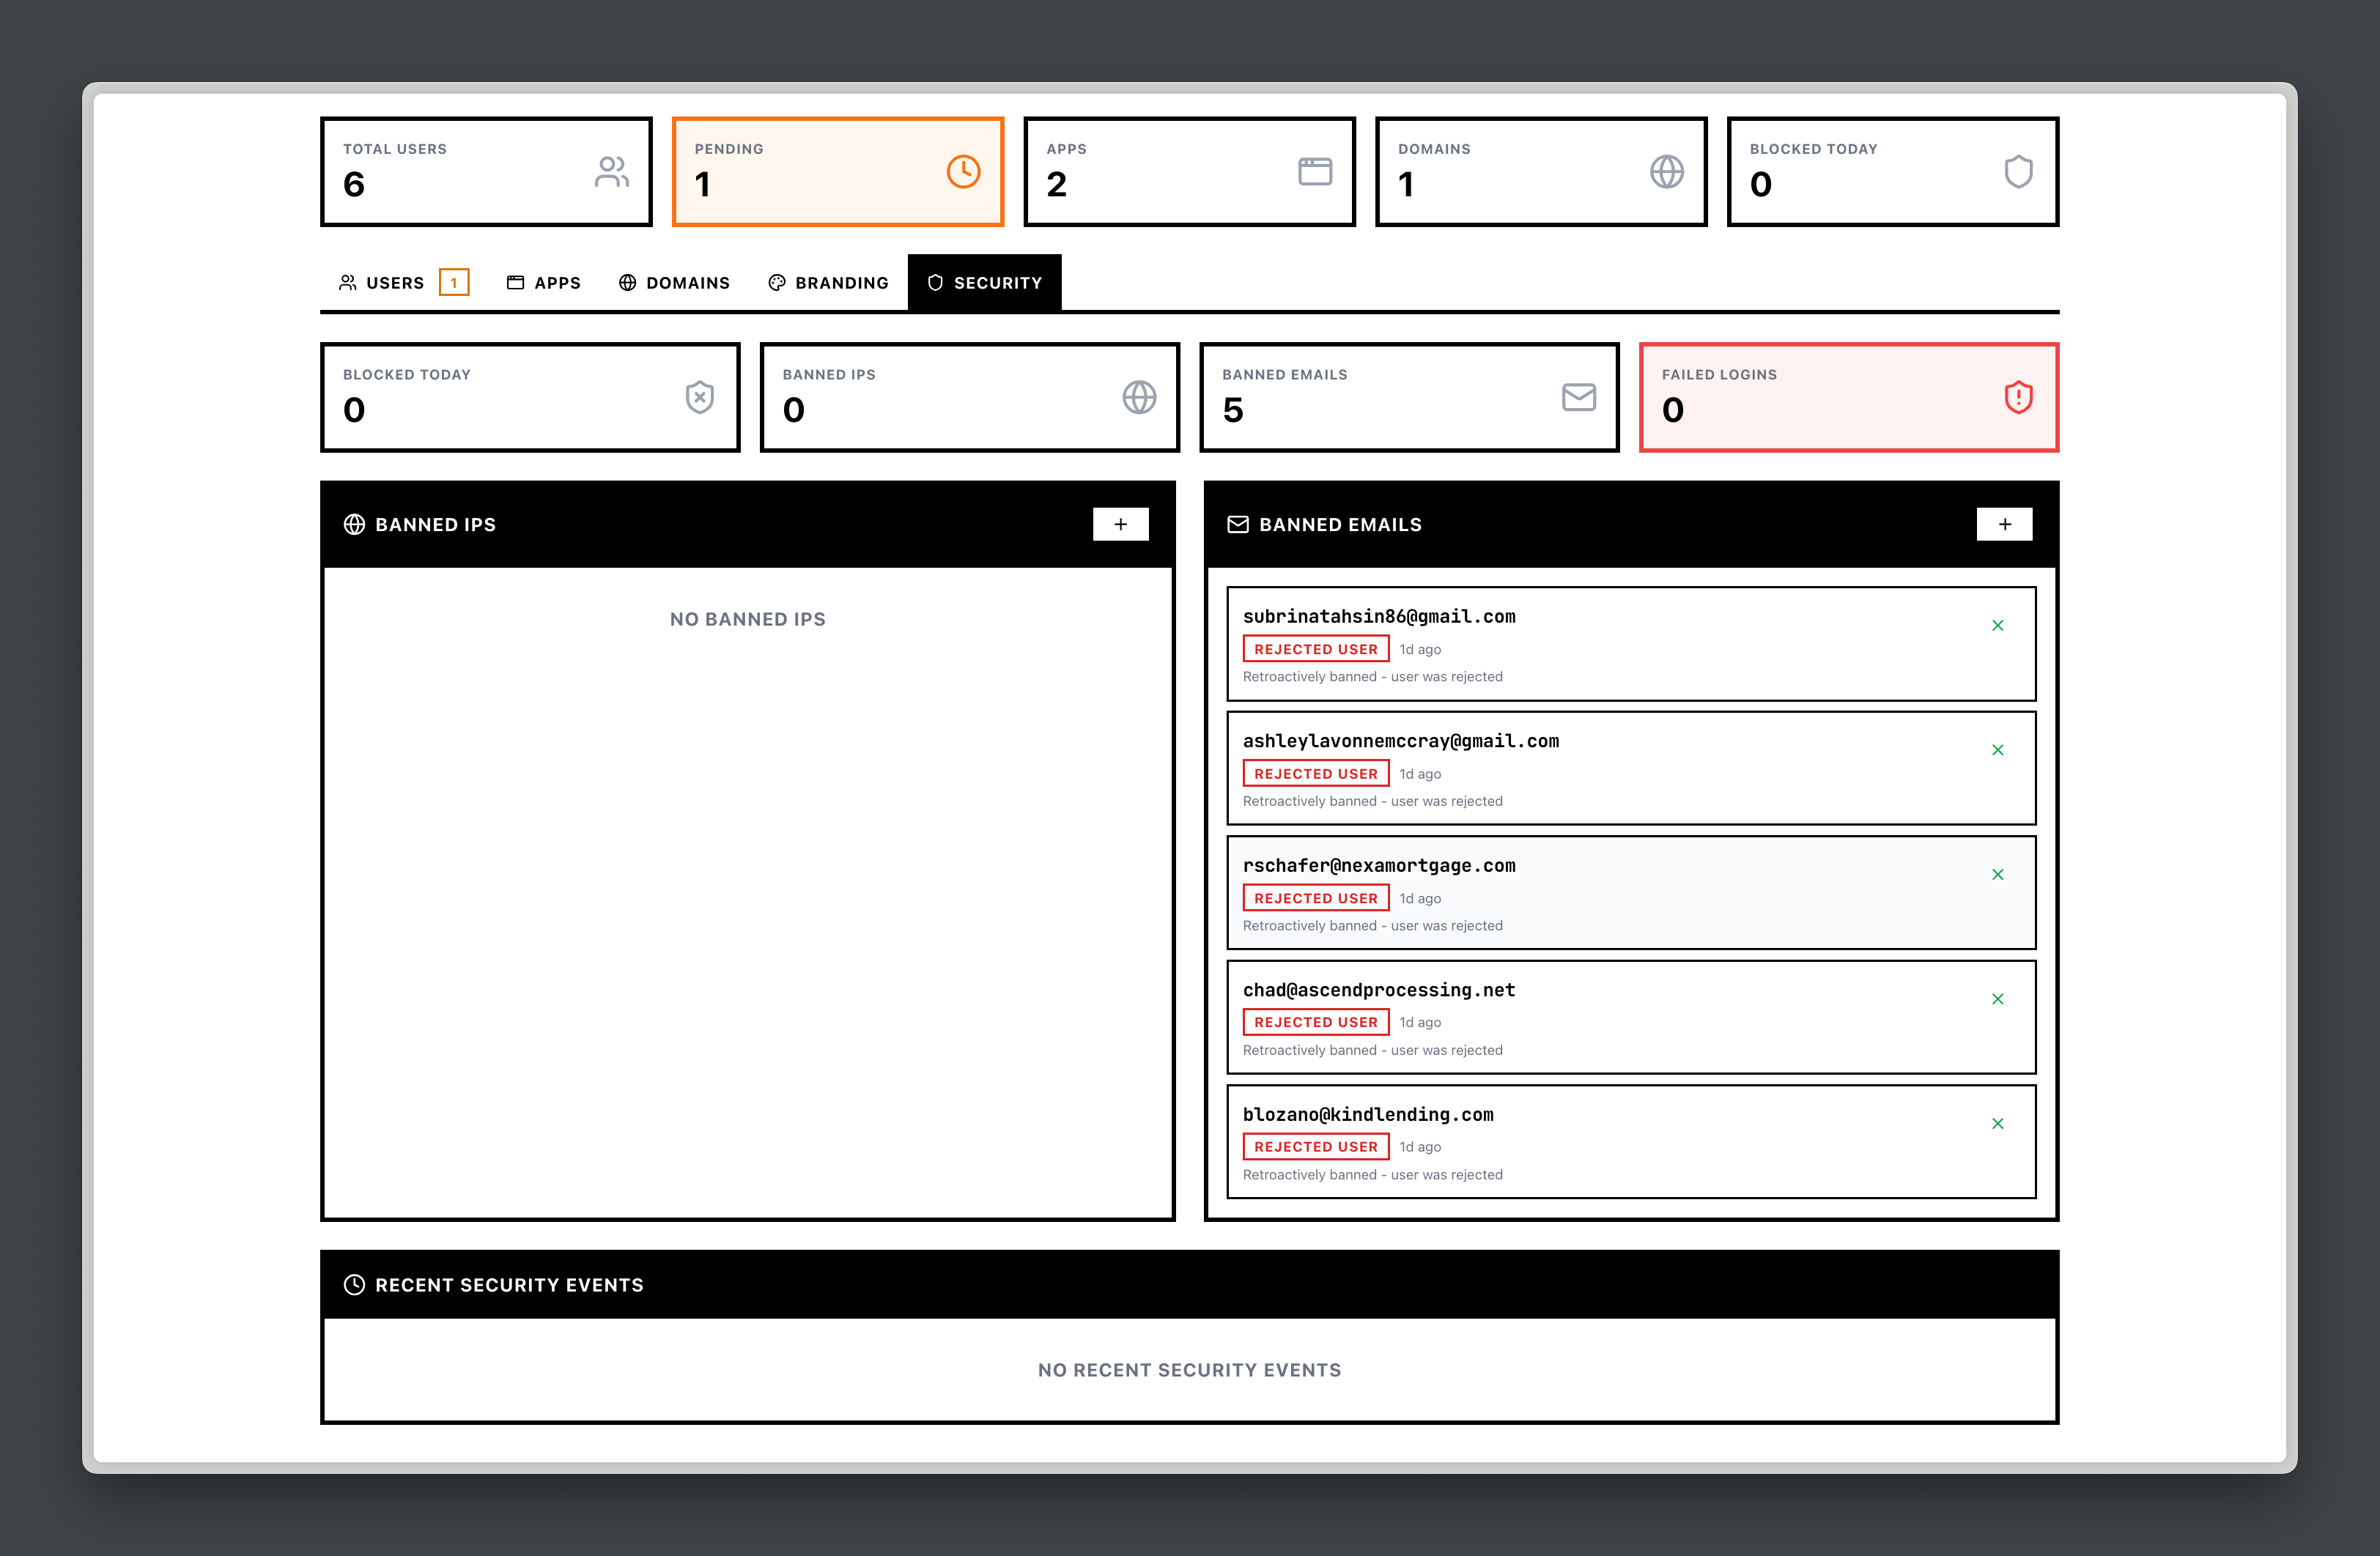
\includegraphics[height=0.85\textheight]{images/security screen.png}
\end{frame}

% ============================================
% SECTION 3: PROJECT 2 - POSTHOG (5-6 mins)
% ============================================
\section{Product Feature: PostHog}


\begin{frame}{PostHog: Background}
    \pause
    \begin{itemize}[<+->]
        \item Complex monorepo: Nest, Next.js, TypeScript, Flutter
        \item I'd heard of PostHog a lot but never used it
        \item Needed analytics across multiple stacks
    \end{itemize}
\end{frame}

\begin{frame}[fragile]{The Prompt}
    \small
    \begin{lstlisting}
This is a monorepo using nest/next, TS, and flutter.
I want to implement simple product analytics using
posthog, tracking login, each step of the sample 
submission flow on mobile, lab flow on web, and more.

First, read through the codebase. Then, ELI5 how
posthog works and how you'd implement posthog in
this mono-repo, and what sdks are available and
how they work, and what env variables you need me
to grab from the dashboard.
    \end{lstlisting}

    \vspace{0.5em}
    \normalsize
    \textbf{Result:} Practically one-shot implementation
\end{frame}

\begin{frame}{Interesting}
    \textbf{Found a compile issue in PostHog's Flutter SDK}

    \vspace{1em}
    \begin{itemize}[<+->]
        \item Ran into it while testing
        \item Opened an issue on GitHub, was writing the PR to fix it
        \item PostHog folks resolved it and closed the issue the same day (that was as good an ad as any for posthog)
    \end{itemize}

    \vspace{1em}
    \onslide<+->
    \textit{That fact that it was a contribution meant I actually went through lines of code to find the compile issue. I learnt some specific details about Flutter - a language I started coding in just 6 months ago.}
\end{frame}

% ============================================
% SECTION 4: REFLECTIONS (3-4 mins)
% ============================================
\section{Reflections}

\begin{frame}{What It Does Well (For Me)}
    \begin{itemize}[<+->]
        \item \textbf{Explains before implementing} - I usually say ELI5 your implementation, and only then have it spit out the plan.
        \item \textbf{One-shots common technical patterns} - WebAuthn/Passkey Support, Google SSO, PostHog Analytics, etc.
        \item I feel a lot less guilt building a project on a new stack because I'm able to (1) check if it's the right project to experiment with the stack much faster, and (2) I can also migrate a lot easier if I need to.
    \end{itemize}
\end{frame}

\begin{frame}{What else has been great}
    \begin{itemize}[<+->]
        \item I used to be a perfectionist; I'd wait to have a perfect plan before starting to implement. This shift has, in many ways, forced me to just build iteratively.
        \item It's also been great for DevOps related debugging. AWS!
    \end{itemize}
\end{frame}

\begin{frame}{What Hasn't Worked}
    \begin{itemize}[<+->]
        \item \textbf{CI/CD:} Wrote a GitHub Action to build docker images on server instead of in CI
        \item \textbf{DRY:} Tends toward repetition, needs nudging to be more DRY, and reviews at the end of each feature
        \item \textbf{UI consistency:} Needs additional \textit{skills} (and often human eye as well) to be consistent/catch issues
    \end{itemize}
\end{frame}

\begin{frame}{What's been changing beyond the code for me}
    \begin{itemize}[<+->]
        \item Team members and users - especially those who didn't code - are much faster at feedback and iterations
        \item So smaller issues that would have been blocked for days are now getting fixed in hours
        \item At the same time, expectations for TaT for fixes is accelerating. That's a tough balance that we're still figuring out.
        \item Older products that we'd built for specific manual analyses are not sufficient - they're not built to sustain heavy querying by an AI agent, for e.g.
        \item It's making me think and spend a lot more time on "what is the product" and "what does it mean to learn"
    \end{itemize}
\end{frame}

\begin{frame}{The Existential Question(s)}
    \Large
    What does it even mean to be a "junior" developer anymore?

    \vspace{1em}
    \normalsize
    How does one grow? What will the "market" appreciate 2-3 years from now - with the rapid acceleration in the field?

    \vspace{1em}
    \textit{Maybe it's judgement and system design/architecture - that's the common refrain we hear. But nothing feels certain anymore, and that is just the reality we're having to reckon with.}

\end{frame}

% ============================================
% CLOSING
% ============================================
\section{End}

\begin{frame}{Thanks for Listening!}
    \begin{center}
        \Large
        Fin.

        \vspace{1em}

        \normalsize

        This presentation is available at: \url{saisneha.com/links/ttt-2026-03}
    

    \vspace{2em}
    \scriptsize
    \url{hello@saisneha.com} \textbar\ \url{saisneha.com} \textbar\ \url{github.com/snehasaisneha}

    \end{center}
\end{frame}

\end{document}
